\documentclass[11pt,a4paper,onecolumn,notitlepage]{article}


%!TEX root = proposal.tex
% Packages
\usepackage[show]{chato-notes}
\usepackage{url}
\usepackage{hyperref}
\usepackage{graphicx}
\usepackage{multirow}
\usepackage{amssymb}
\usepackage{amsmath}
\usepackage{centernot}
% avoid conflicts
\let\proof\relax
\let\endproof\relax
\usepackage{amsthm}
\usepackage{algorithm}
\usepackage{algorithmicx}
\usepackage[noend]{algpseudocode}
\usepackage{enumerate}
\usepackage[dvipsnames]{xcolor}
\usepackage{colortbl}
\usepackage[style=base]{caption}
\usepackage{subcaption}
\usepackage{comment}
\usepackage{balance}
\usepackage{cite} %citations are ordered by number
\usepackage[tikz]{bclogo}
\usepackage[normalem]{ulem}
\usepackage{tikz}
\usepackage{nccmath}
\usepackage{enumitem}
\usepackage{balance}
\usepackage{rotating}
\usepackage{pifont}
\usepackage[margin=2cm]{geometry}
\usepackage{etoolbox} % Patch the bibliography title
\usepackage[noindentafter]{titlesec}

\usetikzlibrary{decorations.markings}
%%
%% The next line says how the "vertex" style of nodes should look: drawn as small circles.
\tikzstyle{vertex}=[circle, draw, inner sep=0pt, minimum size=4pt, fill=black]
\newcommand{\vertex}{\node[vertex]}


\hypersetup{
%    bookmarks=true,         % show bookmarks bar?
    unicode=false,          % non-Latin characters in Acrobats bookmarks
    pdftoolbar=true,        % show Acrobats toolbar?
    pdfmenubar=true,        % show Acrobats menu?
    pdffitwindow=false,     % window fit to page when opened
    pdfstartview={FitH},    % fits the width of the page to the window
    pdftitle={My title},    % title
    pdfauthor={Author},     % author
    pdfsubject={Subject},   % subject of the document
    pdfcreator={Creator},   % creator of the document
    pdfproducer={Producer}, % producer of the document
    pdfnewwindow=true,      % links in new window
    colorlinks=true,       % false: boxed links; true: colored links
    linkcolor=black,          % color of internal links
    citecolor=black,        % color of links to bibliography
    filecolor=black,      % color of file links
    urlcolor=black,           % color of external links
}



\newcommand*{\graphpair}[2]{\langle #1, #2 \rangle}
\newcommand*{\tuple}[1]{(#1_1, ..., #1_n)}
\newcommand*{\range}[3]{#1 = #2 ... #3}
\newcommand*{\pair}[2]{(#1,#2)}
\newcommand*{\triple}[3]{(#1,#2,#3)}
\newcommand*{\edge}[4]{#1 \overset{#3}{#4} #2}
\newcommand*{\uedge}[2]{\edge{#1}{#2}{}{--}}
\newcommand*{\dedge}[2]{\edge{#1}{#2}{}{\rightarrow}}
\newcommand*{\luedge}[3]{\edge{#1}{#2}{#3}{--}}
\newcommand*{\ldedge}[3]{\edge{#1}{#2}{#3}{\rightarrow}}
\newcommand*{\expgname}[1]{#1^+}
\newcommand*{\expgraph}[3]{\expgname{#1}:\graphpair{#2^+}{#3^+}}


%Paper macros



%Style macros
\renewcommand\abstractname{Summary}
%\patchcmd{\thebibliography}{\section*}{\section}{}{}
\renewcommand{\refname}{Bibliography}

%% Work package styles (DO NOT touch)
\renewcommand\theparagraph{\Alph{paragraph}}
\renewcommand\thesubparagraph{[\Alph{paragraph}\arabic{subparagraph}]}
\titleformat{\paragraph}{\normalfont\large\bfseries}{\theparagraph}{1em}{}
\titleformat{\subparagraph}{\normalfont\normalsize\bfseries}{\thesubparagraph}{1em}{}
\titlespacing*{\subparagraph}{0pt}{3.25ex plus 1ex minus .2ex}{1.25ex plus .1ex}
\newcommand{\workpack}{\paragraph}
\newcommand{\subworkpack}{\subparagraph}

\setcounter{secnumdepth}{5}

%Algorithmic macros
\renewcommand{\algorithmicrequire}{\textbf{Input:}}
\renewcommand{\algorithmicensure}{\textbf{Output:}}
\renewcommand{\algorithmicforall}{\textbf{for each}}
\algdef{SE}[DOWHILE]{Do}{DoWhile}{\algorithmicdo}[1]{\algorithmicwhile\ #1}%

%Complexity macros
\newcommand*{\NP}{$\mathbf{NP}$}
\newcommand*{\NPhard}{$\mathbf{NP}$-hard}
\newcommand*{\NPcomplete}{$\mathbf{NP}$-complete}
\newcommand*{\SPcomplete}{$\mathbf{\#P}$-complete}
\newcommand*{\SPhard}{$\mathbf{\#P}$-hard}
\newcommand*{\bigO}{\mathcal{O}}

% Paragraphs
\newcommand{\spara}[1]{\smallskip\noindent{\bf #1}}
\newcommand{\mpara}[1]{\medskip\noindent{\bf #1}}
\newcommand{\para}[1]{\noindent{\bf #1}}

\newcommand{\blackBox}{$\blacksquare$}



\newcommand{\removed}[1]{
  \colorbox{red!30}{{\scriptsize REMOVED}}
  {\color{red}#1}
}

\newcommand{\del}[1]{
  {\color{red}\sout{#1}}
}


\newcommand{\added}[1]{
{\color{ForestGreen}#1}
}



\begin{document}
\title{Graph mining - WS 2016 - Project Report}



%\institute{}

\date{Due date: 24 January 2017}

\author{
Maxi Fischer, S\"oren Tietb\"ohl\\ 
}


\maketitle



% - Summary of the project
\begin{abstract}
Analysis of the Spotify Artist Network using an ego-based community detection algorithm.
\end{abstract}


\section{Summary of the data}

Spotify is a music streaming platform, hosting over 30 million songs and more than 2 million artists. The artists are associated with each other via the 'related artists' feature. This relation induces a graph, which is the subject of this project.

Because the related artists have to be queried one-by-one from the Spotify API we are only using a subset of the complete graph. Our subgraph is constructed by starting at an arbitrary artist (we chose the "Red Hot Chili Peppers") and then using breadth first traversal. The total number of nodes in the subgraph is 50992, the number of edges is 179425. The 'related artist' relation goes both ways, so its an undirected graph. We can assume that in reality the graph is dynamic, because new songs and thus artists will be added all the time. The nodes are not labelled, but various information on the artist relation can be requested, such as genre and popularity.

Degree Distribution: 
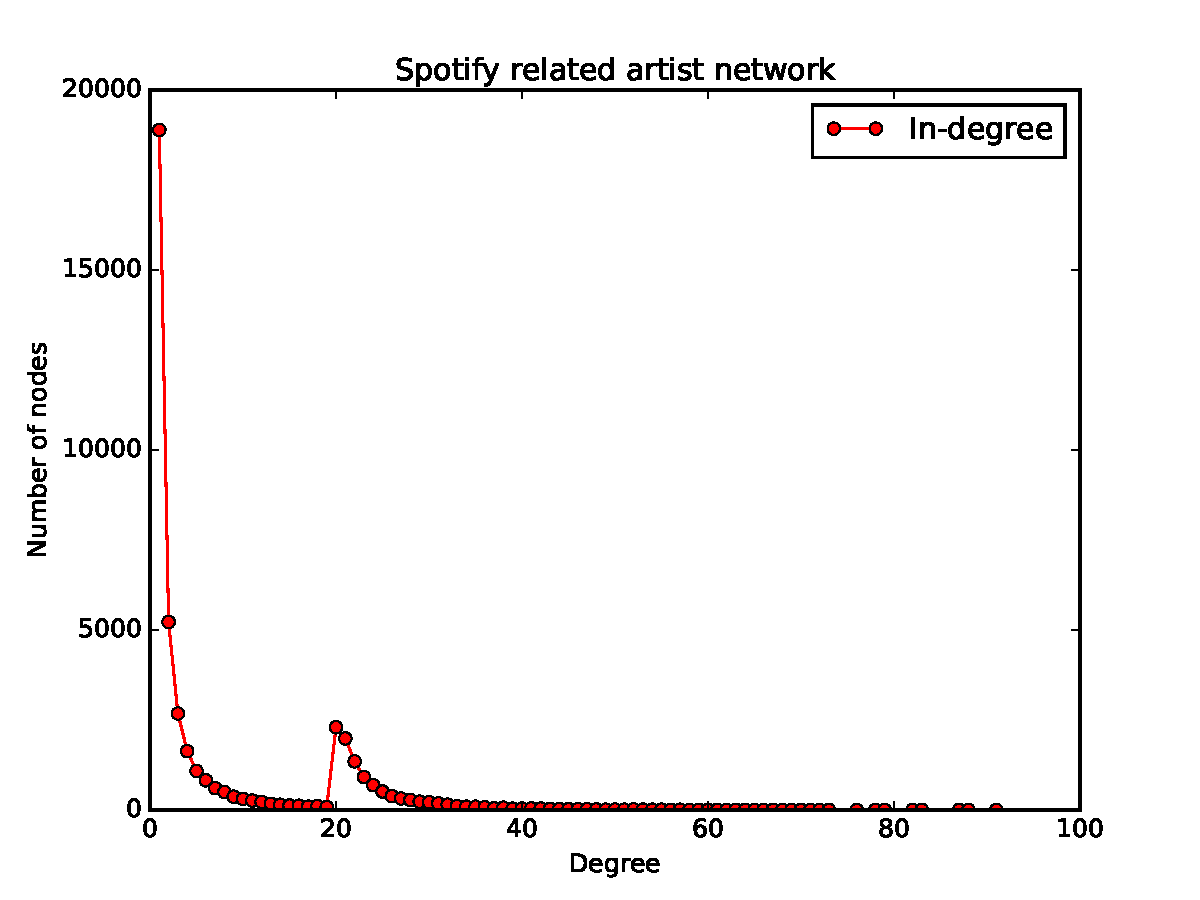
\includegraphics[scale=0.4]{spotify_degree_distribution.pdf}

The number of triangles is 913182. The average clustering coefficient is 0.2536.

\section{Description of the algorithm}

We chose two community detection algorithms: the Louvain-algorithm\cite{louvain} and the k-Clique-Communities\cite{kclique}. For the Louvain algorithm we chose the bestpartition function and for the k-Clique-Communities k = 2 to get the maximum number of partitions.

Briefly, the Louvain algorithms is a hierarchical clustering algorithm that greedy deletes edges that cause high modularity. In the resulting dendogram it chooses the best partition possible of the graph. The Louvain algorithm implementation takes a graph as an input and returns a dictionary with all nodes as keys and their community assignment as values. 

The k-Clique-Communities algorithm looks for all cliques of size k reachable by adjacent k-cliques. It takes the graph as an input and returns a list of sets of nodes, so the communities.

They are both usable on undirectional graphs.

\section{Preprocessing and storing}

In order to obtain the graph we queried the Spotify API at \cite{spotifyapi}. The related artist query returns 20 artists that are related to the given input artist.
From there we continued with breadth first traversal and queried the API for all the new artists.
The nodes are named by the artists id on spotify, which is returned by the API.
Additionally we also store all the artist related information (e.g. genre, popularity etc) in a dictionary that maps from artist id to artist info.
The graph is then written to disk as an adjacency list in plain text. The artist information is stored in json format.

Before the algorithms are run, they will load all the stored information into main memory. This is done to save time, as rebuilding the graph via API takes a long time.

Report all the preprocessing steps to obtain the final network. How do you store the data (graph database, main memory, disk)? In which format? Did you have to remove some information in order to clean the data? 

\section{Network analysis}
Our goal was the community detection in the graph to check the resulting communities against the genre distribution of the artists. We wanted to evaluate which community detection algorithm obtains the best genre-consistent communities. That knowledge is useful to find anomalies in the existing genre assignment and to predict the genre of an artist in the same community. Genre Prediction of songs is a complex research topic in Music Information Retrieval. By using the existing assignment of the Spotify artist relations, we can simplify this prediction.

At first, we calculated the communities with the given algorithms. We analysed the number of artists, null values (artists without an assigned genre) and the genre distribution in a community.

In this section, explain thoroughly the steps of the analysis you performed and give a motivation for such an analysis (e.g. discovering the most influential node, finding interesting patterns, analyzing communities). Elaborate on why you find it challenging and useful. Report possible applications.  

\subsection{Qualitative Results}

We looked at the accuracy of the calculated communities by the algorithms. The accuracy is the number of the most present genre in the community divided by all artists in the community without artists with no genre. The goal is to get informations about the genre consistency of a community. If every artist of a community is part of the most frequent genre, you can say that the whole community is part of this genre.

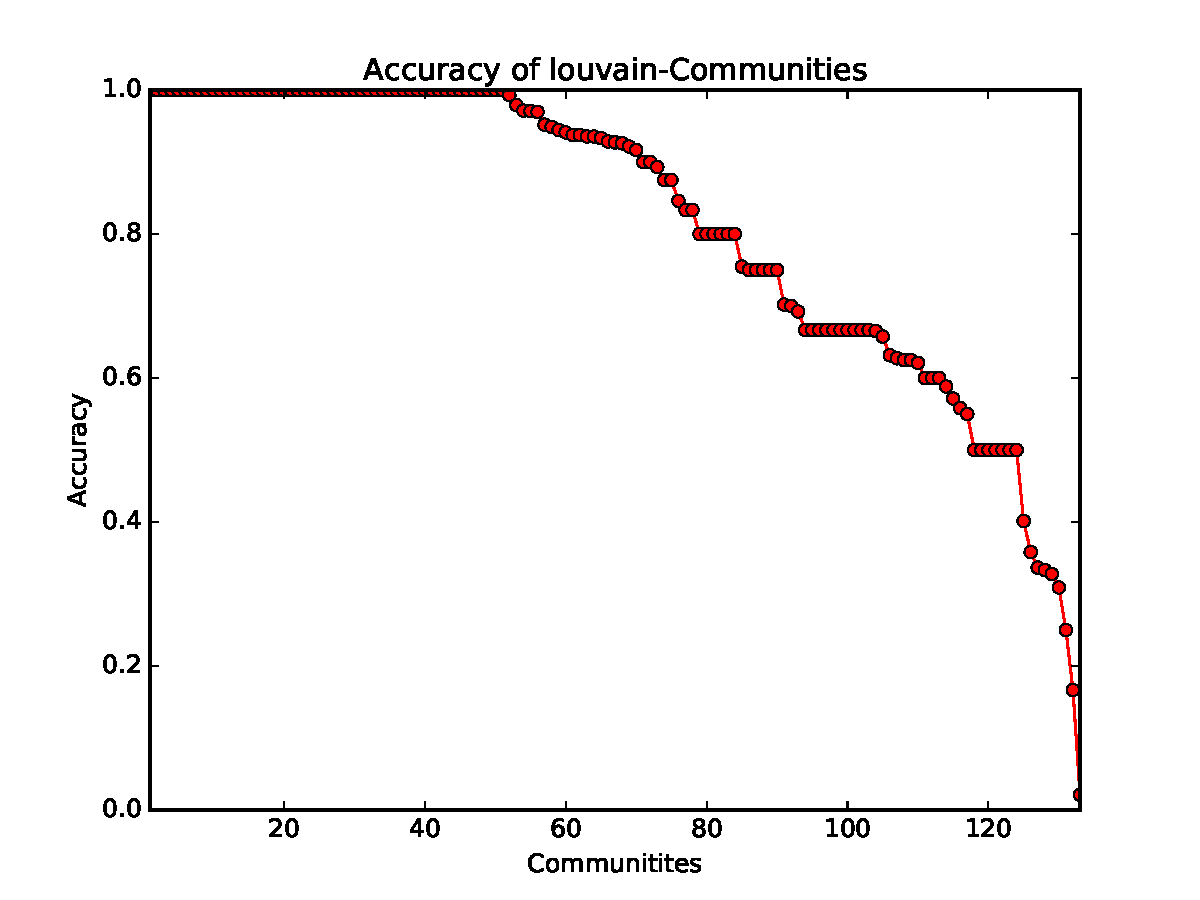
\includegraphics[scale=0.4]{spotify_acc_louvain.pdf}

In the result of the Louvain algorithm most of the communities are relatively high, so that the communities are pretty consistent.

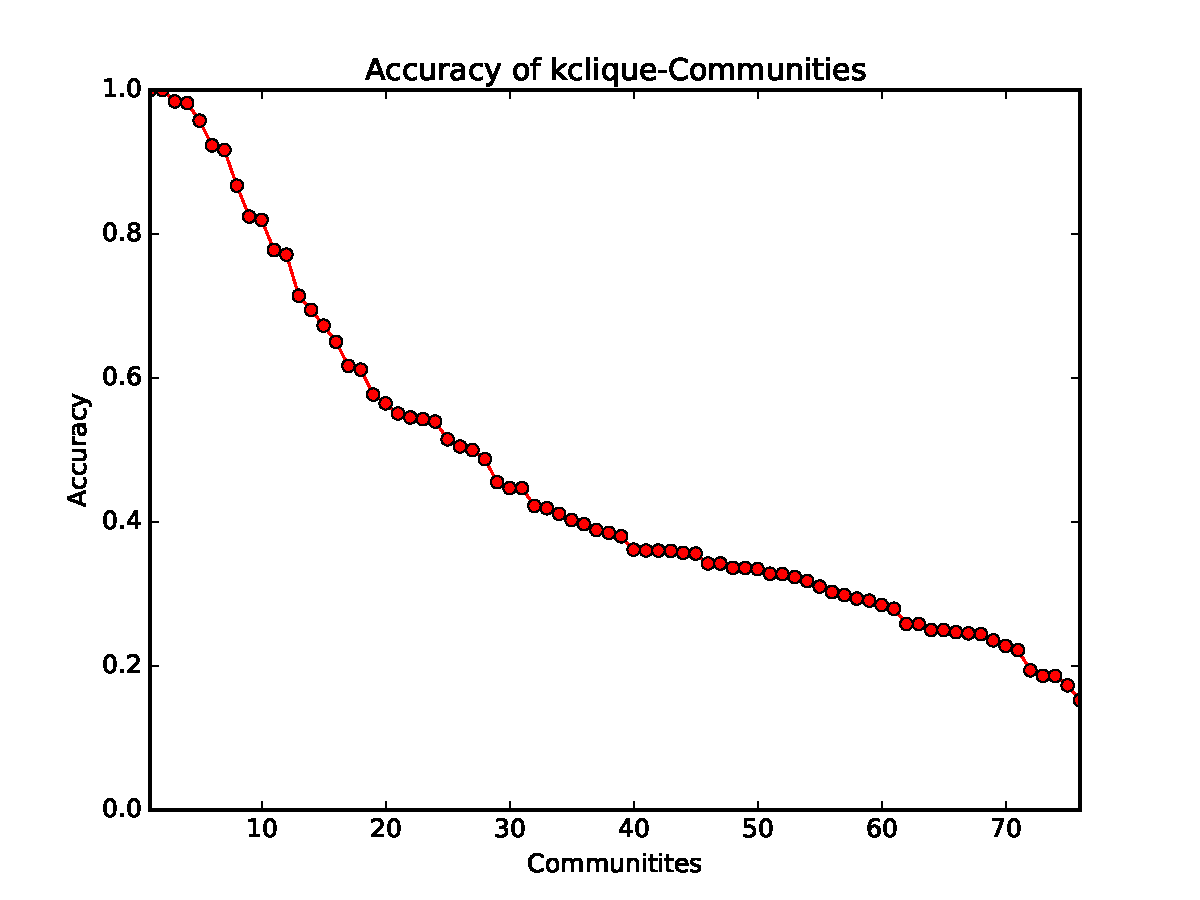
\includegraphics[scale=0.4]{spotify_acc_kclique.pdf}

In comparison the k-Clique-Communities algorithm with k = 2 has many communities with mixed genres. For this use case the detected communities are not very useful.

Then we analysed the number of null values in all calculated communities. We want to find out how much artists have no genre and can be predicted.

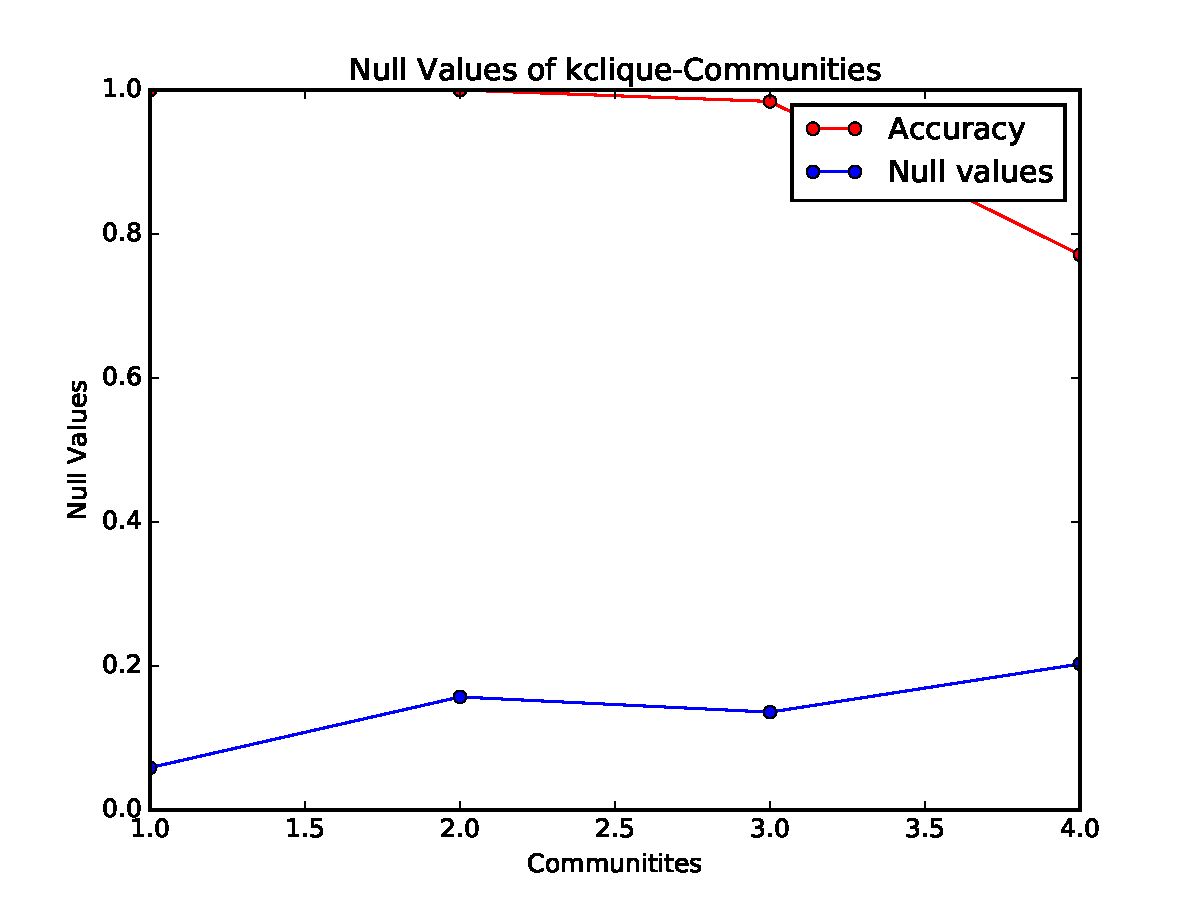
\includegraphics[scale=0.4]{spotify_null_kclique.pdf}

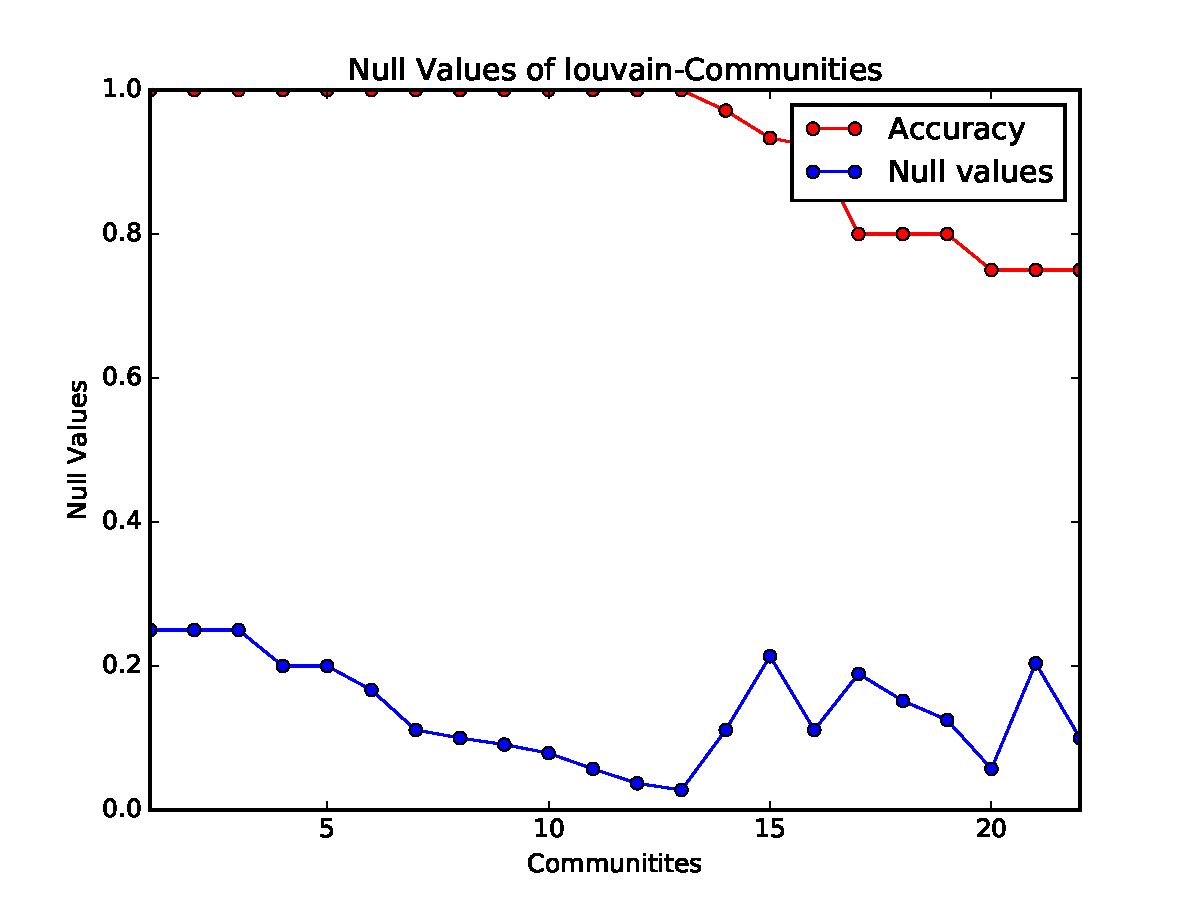
\includegraphics[scale=0.4]{spotify_null_louvain.pdf}

We chose thresholds to predict in how much communities it is useful to predict genres of null_values. The accuracy threshold was 75\%, the null values threshold (number of null values divided by the total number) was 25\%. The accuracy threshold should ensure that there are enough deciding reference points for the prediction while the null values threshold cuts the communities that try to predict too much genres of null values which become much more unclear with more null values. We cut communities with no null values too, because you cannot predict any genres in them.

In the graphics you see the thresholded communities of both algorithms. While Louvain calculated more than 20 communities where you can predict the new genres, 2-Clique-Communities just found 4 communities.

As you may see the Louvain algorithm works much better in that use case. In general it calculates bigger communities that seem to map better on the general genre distribution. 


\subsection{Time and scalability}

\subsubsection*{Building the Graph}

The total amount of time it took to build the graph is 14 minutes 3 seconds. This includes querying the spotify API for related artists and then storing all the information in the respective data structures.

The artist information has a size of 39 MB, the graph adjacency list has a size of 4.8 MB.

\subsubsection*{Running the algorithms}

The Louvain-algorithm completed in 35.6 seconds.

The k-Clique-communitys completed in 92.7 seconds.

Evaluate the used method regarding its run time and scalability. Report the time you need to preprocess  the data (if there is such a phase, like an index construction) and to produce the results. On the same network and algorithm, consider incremental graph sizes (e.g. 10\% of the network, 30\%, etc.). 

\smallskip
\noindent Alternatively, generate some random network with \url{http://www.cse.ust.hk/graphgen/} or any other graph generator and compare the results of the algorithm between the two graphs (the original one and the random one). Are there any important differences in the outcome? Specify the parameters of the graph generator of choice. 


\subsection{[Optional] Memory usage}
Report how much memory is consumed by the algorithm. 


\section{Limitations and interesting findings}

Did you notice any limitation in the approach? Does it work as expected regarding the quality of the results? In terms of performance, is it too slow when the network is too big? Is it domain dependent or applicable to various types of graphs? To which kind of users are the results of the analysis useful? Describe what you have learned and propose ideas on how the analysis could improved. 



% - Bibliography
\bibliographystyle{abbrv}
\bibliography{bibliography}  

\end{document}
